\chapter{Introduction}

\begin{comment}
Andreas
1.1 Domain . . . . . . . . . . . .
1.2 Existing Solutions . . . . . . 
1.3 Task Description . . . . . . . 
1.4 Project Goals . . . . . . . . .
1.4.1 Effect Goals . . . . . . . . 
1.4.2 Result Goals . . . . . . . . 
1.4.3 Learning Goals . . . . . . . 
1.5 Framework . . . . . . . . . . .
1.6 Project Constraints
1.7 Group Background
1.8 Project organization
1.8.1 Responsibilities and roles
1.9 Target Audience 
1.10 Report 
1.10.1 Structure 
\end{comment}

\begin{comment}
sander
1.1 Problem definition . . . . . . .
1.2 Scope of work. . . . . . . . . .
1.3 Requirements and constraints . .
1.4 Goals. . . . . . . . . . . . . . 
1.5 Approach . . . . . . . . . . . .
1.6 Group background and motivation 
1.7 Thesis structure .

Effektmål = Business goal (evt Impact)
Rammer = Framework (føringer fra oppdragsgiver)
Omfang = Scope
Problemområde = Problem area
Begrensninger = Limitations (utenfor din kontroll)
Avgrensninger = Delimitations (noe du bestemmer)
Oppgavedefinisjon = Problem statement ("tese")
\end{comment}

The forestry industry is essential to sustainable resource management, environmental conservation, and economic development. Effective forest management requires expertise in areas such as forest operations, and infrastructure maintenance. To support these efforts, various organizations play a key role in sharing knowledge and providing professional training to uphold best practices.

One such organization is Skogkurs\footnote{\url{https://skogkurs.no/}}, a non-governmental organization established in 1958. The institute operates as a partnership, with 36 forestry organizations and scientific institutions as its members. Its activities are nationwide and encompass a wide range of topics, including forest management, construction and maintenance of forest roads, and forest operations and techniques \cite{skogkurs_eng}. Through its initiatives, Skogkurs aims to enhance the competence of professionals within the forestry industry and to promote knowledge of forests and nature to schools and the general public \cite{skogkurs_nor}. 

\section{Problem Definition}
% Legge til en figur? Evt. fra denne: https://nibio.brage.unit.no/nibio-xmlui/bitstream/handle/11250/3037571/NIBIO_RAPPORT_2022_8_147.pdf?sequence=1
The Nordic forestry industry faces increasing challenges in ensuring stable timber transport throughout the year. Changes in climate have extended the snow-free season, creating variability in forest road conditions due to shifts between frozen, dry, and rainy periods. Addressing these challenges requires digital tools that can assess which forest roads are accessible during different weather conditions.

Recent research has focused on developing methodologies for digitally classifying forest road load-bearing capacities based on soil types and weather conditions. For example, a nationwide pilot study demonstrated that soil types, such as well-drained materials like \gls{glaciofluvial deposit}s, are more suitable for year-round use, while finer sediments require specific conditions like freezing or drying. These findings support the potential for fully digital solutions to predict road accessibility based on a combination of weather patterns and road construction characteristics \cite{fjeld2023trafficability}.

\begin{figure}[h]
    \centering
    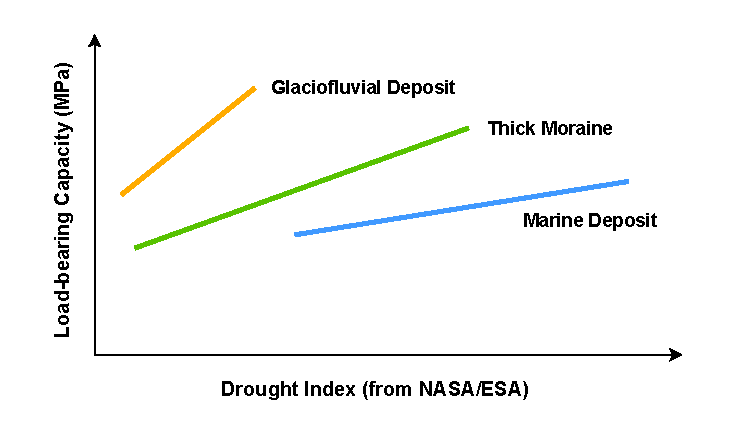
\includegraphics[width=0.7\linewidth]{figures/bæreevne_tørkeindex.pdf}
    \caption[Graph comparing load-bearing capacity to \acrshort{swi}]{Graph comparing load-bearing capacity to \acrshort{swi}, recreated from the task description [\hyperref[appendix:task_description]{Appendix \ref*{appendix:task_description}}]}
    \label{fig:load_to_swi_graph}
\end{figure}

While these studies highlight the feasibility of digital road classification, practical solutions for transport managers remain limited. Current industry practices often rely on experience-based assessments and manual planning, leading to inefficiencies and uncertainty. Although some digital tools have been developed to assist in forest road accessibility assessment, they are not universally applicable across different regions.

\section{Existing Solutions}
% Hva gjør transportledere nå? (spørsmål til usertesting maybe?)

One example is Harvester Seasons\footnote{\url{https://harvesterseasons.com/}}, developed by the Finnish Forest Center, which provides weekly forecasts of road conditions based on soil moisture, temperature, and snow depth. These forecasts use data from sources like \acrshort{nasa}'s \gls{smap} and \acrshort{esa}'s \Gls{sentinel-1} satellites to generate relative load-bearing predictions for winter and snow-free seasons [\hyperref[appendix:task_description]{Appendix \ref*{appendix:task_description}}]. While this tool offers valuable insights, it is limited to Finland and does not provide road condition data for Norway. As a result, it does not meet the needs of Skogkurs, which requires a solution tailored to Norwegian forest roads. This highlights the gap in available tools and the need for a localized approach that accounts for Norway’s specific terrain, climate, and forestry infrastructure.

The current process of scheduling operations for transport managers is based on weather conditions and road \gls{trafficability}. They plan operations either by necessity (e.g., during wet conditions) or by opportunity (e.g., in dry conditions). These decisions are informed by temperature-driven seasonality, regional precipitation patterns, and local knowledge. Additionally, transport lead times and road conditions are influenced by surface deposits and their \gls{permeability}, with difficult weather and reduced road \gls{trafficability} being major challenges in wood supply and transport management \cite{fjeld2023trafficability}. 

\section{Framework}

\textcolor{orange}{NOE TEKST}

\section{Project Organization}

\textcolor{orange}{NOE TEKST}

\section{Thesis Structure}

\textcolor{orange}{NOE TEKST}
